\documentclass[usepdftitle=false,aspectratio=169,usenames,dvipsnames]{beamer}
\usepackage{amsmath, amsfonts, amssymb}
\usepackage{xspace}
\usepackage{xparse}
\usepackage[yyyymmdd]{datetime}
\usepackage{ulem}
\usepackage{array}
\usepackage{multirow}
\usepackage{booktabs}
\usepackage{stmaryrd}
\usepackage{subcaption}
\usepackage{bussproofs}
\usepackage{mathpartir}
\usepackage{minted}
% \usemintedstyle{trac}
\usepackage{xcolor}
\usepackage{proof}

\usepackage{tikz}

\usetikzlibrary{shapes,arrows,positioning,decorations.markings,matrix,fit,calc}
\tikzstyle{line} = [draw, -latex']
\tikzstyle{rline} = [draw, latex'-]
\pgfdeclarelayer{background}
\pgfsetlayers{background,main}
\EnableBpAbbreviations


\DeclareUnicodeCharacter{2265}{$\ge$}
\DeclareUnicodeCharacter{2227}{$\wedge$}
\DeclareUnicodeCharacter{2243}{$\simeq$}
\DeclareUnicodeCharacter{2264}{$\mathbb{\le}$}
\DeclareUnicodeCharacter{2200}{$\mathbb{\forall}$}
\DeclareUnicodeCharacter{2228}{$\vee$}
\DeclareUnicodeCharacter{2084}{$_{4}$}
\DeclareUnicodeCharacter{2083}{$_{3}$}
\DeclareUnicodeCharacter{2082}{$_{2}$}
\DeclareUnicodeCharacter{2081}{$_{1}$}
\DeclareUnicodeCharacter{208A}{$_{+}$}
\DeclareUnicodeCharacter{1D62}{$_{i}$}
\DeclareUnicodeCharacter{208B}{$_{-}$}
\DeclareUnicodeCharacter{03B1}{$\alpha$}

\hypersetup{
  pdftitle={Proving Lean theorems via reconstructed SMT proofs}
  pdfauthor={Tomaz Mascarenhas},
  pdfkeywords={},
  pdfborder={0 0 0}
  draft=false,
  bookmarksnumbered,
  bookmarksdepth=2,
  bookmarksopenlevel=2,
  bookmarksopen
}

\renewcommand{\dateseparator}{--}

%%% BEGIN Defining style
\useinnertheme[outline]{chamfered}
\setbeamertemplate{navigation symbols}{}%remove navigation symbols
\usefonttheme[onlymath]{serif}%beamer math looks like article math
\usecolortheme{seahorse}
\setbeamercolor{palette quinary}{use=structure,fg=black,bg=white}
%%% END Defining style

%%% BEGIN Biblatex for references
\usepackage[backend=bibtex,
doi=false,isbn=false,url=false,
% show initials only
style=alphabetic,
% Show name
% style=authoryear-icomp,
% citation label has 4 initials if up to 4 authors, 3 and "+" otherwise
maxalphanames= 4, maxcitenames = 3, minalphanames = 3, minnames = 3]{biblatex}
% citation label has first author's name et al
% maxcitenames=2,backend=biber]{biblatex}

\bibliography{./refs.bib}

%%%%%%%%%%%%% macros

\mathchardef\mhyphen="2D % Define a "math hyphen"

\usepackage{pifont}

\newcommand{\bluecheck}{{\color{blue}\checkmark}}
\newcommand{\redmark}{\color{red}{\ding{55}}}

\newcommand\vvthinspace{\kern+0.041667em}
\newcommand\vthinspace{\kern+0.083333em}
\newcommand\negvthinspace{\kern-0.083333em}
\newcommand\negvvthinspace{\kern-0.041667em}

\newcommand\FV[1]{\textrm{FV}(#1)}

\newcommand\sym[1]{\mathsf{#1}}

%ADT font macros
\newcommand{\typename}[1]{\mathbf{\mathrm{#1}}}
\newcommand{\consname}[1]{\mathrm{#1}}
\newcommand{\selname}[1]{\mathrm{#1}}
\newcommand{\testername}[1]{\mathrm{#1}}

\newcommand{\SInt}{\typename{Int}}
\newcommand{\SBool}{\typename{Bool}}
\newcommand{\SStr}{\typename{Str}}

\newcommand{\evalfn}[1]{\mathrm{eval}_{#1}}

\DeclareDocumentCommand{\qnt}{ O{n} m O{\psi}}{\innerqnt(#2,#1) #3}
\def\innerqnt(#1,#2,#3){#1 \bar #2.\>}

\DeclareDocumentCommand{\terms}{ m O{}}{\mathbf{T}_{#2}(#1)}

\DeclareDocumentCommand{\bfapp}{ O{f} m O{n}}{#1({\bar #2}_{#3})}
\DeclareDocumentCommand{\enum}{ O{n} m O{,\,} O{} O{1}}{#2_#5#4#3\dots #3#2_{#1}#4}
\DeclareDocumentCommand{\benum}{ O{n} m O{\mapsto} O{} O{,\,} O{1}}{\innerbenum(#2,#3,#6,#4)#5\dots #5\innerbenum(#2,#3,#1,#4)}
\def\innerbenum(#1,#2,#3,#4,#5){#1_{#4}#3 #5{#2_{#4}}}

\DeclareDocumentCommand{\bfenum}{O{\mapsto} m}{\innerbfenum(#2,#1)}
  \def\innerbfenum(#1,#2,#3){\bar #1#3 \bar #2}
\DeclareDocumentCommand{\fapp}{ O{f} m O{n} O{,\,} O{(} O{)}}{#1#5#2_1#4\dots #4#2_{#3}#6}

% Column that takes width (left justified): L{1cm}, e.g.
\newcolumntype{L}[1]{>{\raggedright\arraybackslash$} p{#1} <{$}}

% Column with math mode in displaystyle
\newcolumntype{F}[1]{>{$\displaystyle} #1 <{$}}

% Column with math mode in displaystyle
\newcolumntype{D}[1]{>{\displaystyle} #1 <{}}

% Allows to break like in cell; first arg is $t,b,c$, for alignment with other cells
\newcommand{\specialcell}[2][c]{%
  \begin{tabular}[#1]{@{}l@{}}#2\end{tabular}}

\newcommand{\ccfv}{\textsc{CCFV}}

% \newcommand{\cdclt}{CDCL($\mathcal{T}$)}
\newcommand{\cdclt}{CDCL(T)}
\newcommand{\dpllt}{\cdclt}

\newcommand{\cvcho}{\textsc{cvc}4-\textsc{ho}\xspace}
\newcommand{\cvc}{\textsc{cvc}4\xspace}
\newcommand{\zzz}{Z3}
\newcommand{\verit}{\textsc{veriT}\xspace}

\newcommand{\basestrat}[1]{{\bf #1}}
\newcommand\interleavestrat[2]{\basestrat{#1}+\basestrat{#2}}
\newcommand\mathinterleavestrat[2]{$\mathbf{#1}$+$\mathbf{#2}$}
\newcommand\prioritystrat[2]{\basestrat{#1};\basestrat{#2}}
\newcommand{\zbasestrat}[1]{{\bf z3 #1}}
\newcommand{\zprioritystrat}[2]{{\bf z3} \basestrat{#1};\basestrat{#2}}
\newcommand{\E}{\mathsf{E}}
\newcommand{\Q}{\mathsf{Q}}
\newcommand{\M}{\mathsf{M}}
\newcommand{\ite}{\mathsf{ite}}
\newcommand{\Mod}{\mathcal{M}}
\newcommand{\termordereq}{\preceq}
\newcommand{\termorder}{\prec}
\newcommand{\teq}{\simeq}
\newcommand{\tneq}{\not\simeq}

\newcommand{\inputform}{\psi}
\newcommand{\matrixform}{\varphi}

\newcommand\vitem{\vfill\item}
\newcommand\pvitem{\pause\vfill\item}
\newcommand\pitem{\pause\item}

\newcommand{\cvcsy}{\textsc{cvc}4\textsc{sy}\xspace}
\newcommand{\cvccegis}{\textsc{cvc+c}\xspace}
\newcommand{\cvcu}{\textsc{cvc+upi}\xspace}
\newcommand{\cvcuci}{\textsc{cvc+upi+e}\xspace}
\newcommand{\cvcport}{\textsc{cvc-port}\xspace}
\newcommand{\loopinv}{\textsc{loopinvgen}\xspace}

\newcommand{\divc}{D\&C\xspace}

% AJR : update these
\newcommand{\unif}{Unif+PI\xspace}
\newcommand{\unifci}{Unif+PI+E\xspace}
\newcommand{\smtclass}{\textsc{SMTClassify}\xspace}
\newcommand{\learn}{\textsc{Learn}\xspace}
\newcommand{\classchecker}{\textsc{ClassChecker}\xspace}

%%%%%%%%%%%%


% To avoid number in slides that break, like the references one
\setbeamertemplate{frametitle continuation}{}

% Small font
\renewcommand*{\bibfont}{\scriptsize}
%%% END Biblatex for references



%%% BEGIN DEFINING TITLE PAGE

\defbeamertemplate{title page}{mystyle}[1][]
{
  \vbox{}
  \vfill
  \begingroup
    \centering
    {\usebeamercolor[fg]{titlegraphic}\inserttitlegraphic\par}
    \vskip1em
    \begin{beamercolorbox}[sep=0pt,center,#1,rounded=true,wd=10cm]{title}
      \usebeamerfont{title}\inserttitle\par%
      \ifx\insertsubtitle\@empty%
      \else%
        \vskip0.25em%
        {\usebeamerfont{subtitle}\usebeamercolor[fg]{subtitle}\insertsubtitle\par}%
      \fi%
    \end{beamercolorbox}%
    \vskip1em\par
    \begin{beamercolorbox}[sep=8pt,center,#1]{author}
      \usebeamerfont{author}\insertauthor
    \end{beamercolorbox}
    \begin{beamercolorbox}[sep=8pt,center,#1]{institute}
      \usebeamerfont{institute}\insertinstitute
    \end{beamercolorbox}
    \begin{beamercolorbox}[sep=0pt,center,#1]{date}
      \usebeamerfont{date}\insertdate
    \end{beamercolorbox}%
  \endgroup
  \vfill
}

\setbeamertemplate{title page}[mystyle]

%%% END DEFINING TITLE PAGE

%%% BEGIN Meta information
\author[Tomaz Mascarenhas]
{%
  \texorpdfstring{
    Tomaz Mascarenhas\\Advisor: Haniel Barbosa\\
      \vspace{3ex}
    \begin{columns}
      \column{.45\linewidth}
        \centering
        
\includegraphics[height=0.25\textheight]{images/DCC_LOGO.jpg}
      \column{.35\linewidth}
        
\includegraphics[height=0.15\textheight]{images/Logo_UFMG.jpg}
        % \vspace{2ex}
      %   \centering
      %   
\includegraphics[height=0.15\textheight]{images/DCC_LOGO.jpg}
    \end{columns}
  }
  {}
}

\date{Belo Horizonte, Brazil, 2023/09/12}

\title[Proving Lean theorems via reconstructed SMT proofs]{Proving Lean theorems via reconstructed\\SMT proofs}

% Redifining footer
\makeatother
\setbeamertemplate{footline}
{
  \leavevmode%
  \hbox{%
    \begin{beamercolorbox}[wd=.6\paperwidth,ht=2.5ex,dp=1ex,left]{title in head/foot}%
      {\hspace{1em}\usebeamerfont{title in head/foot}\insertshorttitle}
    \end{beamercolorbox}%
    \begin{beamercolorbox}[wd=.2\paperwidth,ht=2.5ex,dp=1ex,left]{title in head/foot}%
      {\hspace{1em}\usebeamerfont{title in head/foot}Tomaz Mascarenhas, UFMG}
    \end{beamercolorbox}%
    \begin{beamercolorbox}[wd=.2\paperwidth,ht=2.5ex,dp=1ex,right]{title in head/foot}%
      \insertframenumber{} / \inserttotalframenumber\hspace{1em}
    \end{beamercolorbox}}%
  \vskip0pt%
}
\makeatletter
%%% END Meta information

%%% BEGIN Tikz setup
\usepackage{tikz}
\usetikzlibrary{positioning,calc,intersections,backgrounds, fadings}
\usetikzlibrary{shapes}

  \tikzset{
    invisible/.style={opacity=0},
    visible on/.style={alt=#1{}{invisible}},
    alt/.code args={<#1>#2#3}{%
      \alt<#1>{\pgfkeysalso{#2}}{\pgfkeysalso{#3}} % \pgfkeysalso doesn't change the path
    },
  }

\definecolor{BloodRed}{rgb}{.86,0,0}
\definecolor{gold(metallic)}{rgb}{0.83, 0.69, 0.22}

\definecolor{procColor}{rgb}{0.628,0.35,0.17}
\definecolor{cnfColor}{rgb}{0.82, 0.0, 0.86}
% \definecolor{cnfColor}{rgb}{.83,.66,0}
\definecolor{satColor}{rgb}{.83,0,0}
\definecolor{thSolverColor}{rgb}{0,.5,0}
\definecolor{thRwColor}{rgb}{0,0,1}
\definecolor{thCombColor}{rgb}{0.5,0.5,0}

% spec
\definecolor{spec}{rgb}{0.0, 0.0, 0.86}
% syntax recstrictions
\definecolor{grammar}{rgb}{0.82, 0.0, 0.86}

\tikzfading[
  name=arrowfading,
  top color=transparent!0,
  bottom color=transparent!95
]
\newcommand*{\tikzarrow}[2]{%
  \tikz[
    baseline=(A.base),             % Set baseline to the baseline of node content
    font=\footnotesize\sffamily    % Set fontsize of the node content
  ]
  \node[
    single arrow,                  % Shape of the node
    single arrow head extend=4pt,  % Actual width of arrow head
    single arrow tip angle=150,    % Adjust arrow tip angle
    shape border rotate=270,       % Rotate the arrow shape to point down
    draw=red!25,                   % Draw the node shape (with certain border color
    inner sep=2pt,                 % Separation between node content and node shape
    top color=white,               % Shading color on top of node
    bottom color=#1,               % Shading color on bottom of node
    general shadow={               % Specifications for the shadow
      fill=black,
      shadow yshift=-0.5ex,
      path fading=arrowfading
    }
  ] (A) {#2};%
}

%%% END Tikz setup

\newcommand{\qgo}[1]{\innerqgo(#1)}
    \def\innerqgo(#1,#2,#3){#1 #2_1\dots #2_n.~{#3}}
\def\qg#1{\innerqg(#1)}
    \def\innerqg(#1,#2,#3){#1\mathbf{#2}.~{#3}}
\DeclareDocumentCommand{\qgb}{ m O{} }{\innerqgb(#1,#2)}
\def\innerqgb(#1,#2,#3,#4){#1\bar #2_{#4}.~{#3}}
\DeclareDocumentCommand{\fapp}{ O{f} m O{n} O{,} O{(} O{)}}{#1#5#2_1#4\dots #4#2_{#3}#6}
\DeclareDocumentCommand{\fappint}{ O{f} m O{n} O{,}}{\innerfappint(#1,#2,#3,#4)}
  \def\innerfappint(#1,#2,#3,#4,#5,#6){#1(#3#2_1#4#6\dots #6#3#2_{#5}#4)}
\DeclareDocumentCommand{\bfapp}{ O{f} m O{}}{#1(\bar {#2}_{#3})}

\DeclareDocumentCommand{\enum}{ O{n} m O{,} O{} O{1}}{#2_#5#4#3\dots #3#2_{#1}#4}
\DeclareDocumentCommand{\benum}{ O{n} m O{\mapsto} O{} O{,\,} O{1}}{\innerbenum(#2,#3,#6,#4)#5\dots #5\innerbenum(#2,#3,#1,#4)}
  \def\innerbenum(#1,#2,#3,#4,#5){#1_{#4}#5#3 {#2_{#4}}#5}

\usepackage{soul,xcolor}

\setstcolor{red}
\makeatletter
\newcommand\SoulColor{%
  \let\set@color\beamerorig@set@color
  \let\reset@color\beamerorig@reset@color}
\makeatother

\DeclareDocumentCommand{\soutthick}{ O{.4pt} m }{%
    \renewcommand{\ULthickness}{#1}%
       \sout{#2}%
    \renewcommand{\ULthickness}{.4pt}% Resetting to ulem default
}

\definecolor{ao}{rgb}{0.0, 0.0, 1.0}
\definecolor{ao(english)}{rgb}{0.0, 0.5, 0.0}
\definecolor{asparagus}{rgb}{0.53, 0.66, 0.42}
\definecolor{bostonuniversityred}{rgb}{0.8, 0.0, 0.0}
\definecolor{darkbrown}{rgb}{0.4, 0.26, 0.13}
\definecolor{alizarin}{rgb}{0.82, 0.1, 0.26}
% 2952bfff
\definecolor{ceruleanblue}{rgb}{0.16, 0.32, 0.75}
% 8c008cff
\definecolor{darkmagenta}{rgb}{0.55, 0.0, 0.55}
% #8FBC8F
\definecolor{darkseagreen}{rgb}{0.56, 0.74, 0.56}

\usepackage{tikz-qtree}

%%%%%%%%%%%%%%%% BEGIN define outline machinery

\newcommand{\beamersec}[2]{%
  \section*{#1}
  \addcontentsline{toc}{section}{$\bullet$ #1 \vspace{10pt}\newline  \includegraphics[height=.3\textheight]{#2}\vfill}

  \begin{frame}
    \vfill
    \begin{center}
      \vfill\textbf{#1}\vfill
      \includegraphics[height=.5\textheight]{#2}
      \vfill
    \end{center}
    \vfill
  \end{frame}
}

\newcommand{\beamersubsec}[1]{%
  \subsection*{#1}
  \addcontentsline{toc}{section}{$\mbox{}\quad-$ #1 \vspace{10pt}\newline\vfill}

  \begin{frame}
    \vfill
    \begin{center}
      \textbf{#1}
    \end{center}
    \vfill
  \end{frame}
}

\newcommand{\beamersubsubsec}[1]{%
  \subsection*{#1}
  \addcontentsline{toc}{section}{$\mbox{}\qquad\cdot$ #1 \vspace{10pt}\newline\vfill}
}

%%%%%%%%%%%%%%%% END define outline machinery

%%% BEGIN trick for not counting references

\newcommand{\backupbegin}{
   \newcounter{framenumberappendix}
   \setcounter{framenumberappendix}{\value{framenumber}}
}
\newcommand{\backupend}{
   \addtocounter{framenumberappendix}{-\value{framenumber}}
   \addtocounter{framenumber}{\value{framenumberappendix}}
}

%%% END trick for not counting references

\newcommand{\red}[1]{\textcolor{red}{#1}}

% Creating boxes with width of given text; first parameter (optional) is
% alignment of box, then text to be taken the width, then the text to be boxed
\newlength\stextwidth
\newcommand\makesamewidth[3][c]{%
  \settowidth{\stextwidth}{#2}%
  \makebox[\stextwidth][#1]{#3}%
}

% color highlight
% f0dc9cff

\AtBeginSection[]{
  {
    \setbeamertemplate{footline}{}
  \begin{frame}
  \vfill
  \centering
  \begin{beamercolorbox}[sep=8pt,center,shadow=true,rounded=true]{title}
    \usebeamerfont{title}\insertsectionhead\par%
  \end{beamercolorbox}
  \vfill
\end{frame}
}
\addtocounter{framenumber}{-1}
}

% Theorem settings
\addtobeamertemplate{theorem begin}{%
  \setbeamercolor{block title}{fg=white,bg=black}%
  \setbeamercolor{block body}{fg=black, bg=white!90!black}%
}{}

%%% BEGIN CHANGING BULLETS STYLE

\setbeamertemplate{itemize item}{$\vartriangleright$}
\setbeamertemplate{itemize subitem}{$\blacktriangleright$}
\newlength\origleftmargini
\setlength\origleftmargini\leftmargini
\newlength\origleftmarginii
\setlength\origleftmarginii\leftmarginii
\setlength\leftmargini{1em}
\setlength\leftmarginii{1.25em}
\setlength\leftmarginiii{1em}

%%% END CHANGING BULLETS STYLE

\setbeamersize{text margin left=1em, text margin right=1.5em}

\newcommand{\yell}[1]{{\textcolor{red}{[#1]}}}

\newcommand{\cvcc}{\textsc{cvc}{\small 4}\textsc{sy}\textsc{+b}\xspace}
\newcommand{\cvca}{\textsc{cvc}{\small 4}\textsc{sy}\textsc{+u}\xspace}
\newcommand{\gpid}{\textsc{GPiD}\xspace}
\newcommand{\explain}{\textsc{Explain}\xspace}

\newcommand{\mysetminusD}{\hbox{\tikz{\draw[line width=0.6pt,line cap=round] (3pt,0) -- (0,6pt);}}}
\newcommand{\mysetminusT}{\mysetminusD}
\newcommand{\mysetminusS}{\hbox{\tikz{\draw[line width=0.45pt,line cap=round] (2pt,0) -- (0,4pt);}}}
\newcommand{\mysetminusSS}{\hbox{\tikz{\draw[line width=0.4pt,line cap=round] (1.5pt,0) -- (0,3pt);}}}

\newcommand{\mysetminus}{\mathbin{\mathchoice{\mysetminusD}{\mysetminusT}{\mysetminusS}{\mysetminusSS}}}

\def\vv{\smallskip}

\newcommand{\sep}{~\mid~}

\makeatletter
\newcommand\notsotiny{\@setfontsize\notsotiny{7}{8}}
\makeatother

\newcommand\chighlight[2]{\setlength{\fboxsep}{0pt}\colorbox{#1}{#2\strut}}

\begin{document}

{
\setbeamertemplate{footline}{}
\frame{\titlepage}
}
\addtocounter{framenumber}{-1}

\begin{frame}
  \frametitle{History: Computers and Proofs}
  \begin{itemize}
    \item \emph{Four color theorem}: the first major cooperation between humans and computers to prove a theorem
    \vitem Given a map, what is the minimum number of colors necessary to paint each region in a way that no two adjacent regions share the same color?
    \vitem This is equivalent to coloring vertices in \textit{planar} graphs
    \vitem Conjecture: it is always possible to find such a coloring with at most 4 colors
  \end{itemize}
  \centering
  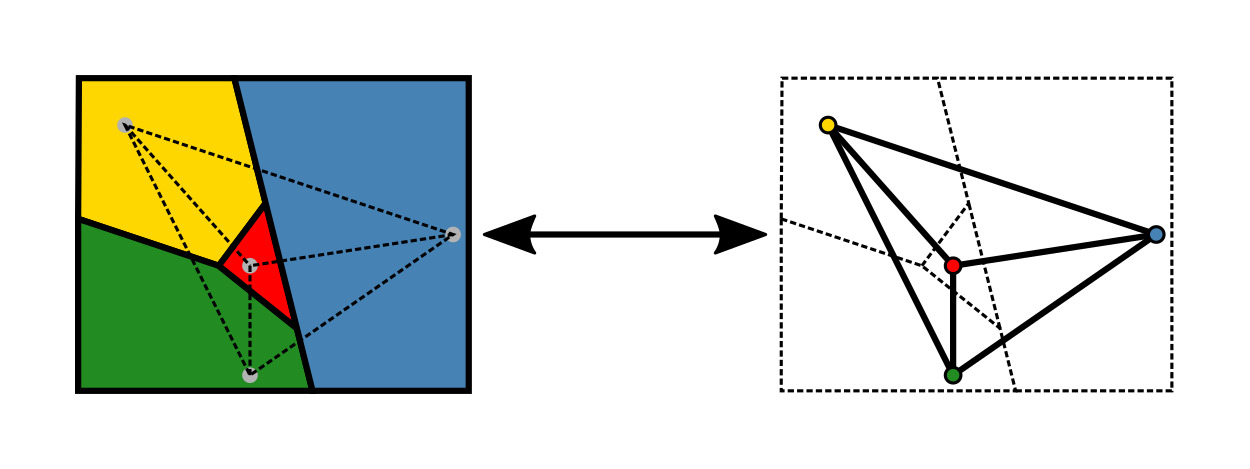
\includegraphics[scale=0.7]{images/fourColor.jpg}
\end{frame}

\begin{frame}
  \frametitle{History: Computers and Proofs}
  \begin{itemize}
    \item The usual technique to prove such a fact is to find an \textit{unavoidable set} and prove that each of its elements is \textit{reducible}
    \vitem For this conjecture, the minimal unavoidable set found had 1834 elements, which was too hard to be checked
    \vitem Mathematicians realized that they could write computer programs to check the reducibility of each graph, instead of doing it manually
    \vitem In 1989, Appel and Hekken proved the theorem using this approach, which created a debate on whether or not this kind of proof is acceptable
  \end{itemize}
\end{frame}

\begin{frame}
  \frametitle{Automatic and Interactive Theorem Provers}

  \begin{itemize}
    \item Nowadays we have more sophisticated tools that promote the cooperation between humans and computers to prove theorems
    \vitem Automatic Theorem Provers (ATPs)
    \begin{itemize}
      \item Define a conjecture and press a button to check its validity
      \item Backend of many systems for verification of software
      \item SMT Solvers (z3, \textbf{cvc5})
    \end{itemize}
    \vitem Interactive Theorem Provers (ITPs)
    \begin{itemize}
      \item Proof production guided by the user
      \item Formalization of mathematics
      \item Twelf, Coq, \textbf{Lean}
    \end{itemize}
  \end{itemize}
\end{frame}

\begin{frame}
  \frametitle{Automatic and Interactive Theorem Provers}
  \begin{table}[]
  \begin{tabular}{|c|c|c|}
  \hline
              & \textbf{Lean}                                & \textbf{cvc5}                          \\ \hline
  Expressivity & Calculus of Inductive Constructions & Many-Sorted First Order Logic \\
  Trusted Base & Small kernel                        & Complete software             \\
  Usage        & Build proofs step by step           & Fully automatic               \\ \hline
  \end{tabular}
  \end{table}
\end{frame}


\begin{frame}
  \frametitle{Automatic and Interactive Theorem Provers}
  \begin{itemize}
    \item Cooperation between ATPs and ITPs via proof certificates
    \vitem Hammers: using ATPs to prove theorems stated in the ITP
    \vitem SMTCoq, Sledgehammer
    \vitem Lean?
  \end{itemize}
\end{frame}

% \begin{frame}
%   \frametitle{Implementing Hammers}
%   \begin{itemize}
%     \item Translation Module
%     \vitem Premise Selection Module
%     \vitem Proof Reconstruction Module
%     \begin{itemize}
%       \item{Certified vs Certifying}
%     \end{itemize}
%   \end{itemize}
% \end{frame}


\begin{frame}
  \frametitle{Implementing Hammers}
  \begin{minipage}[c][0.55 \textheight]{0.45 \textwidth}
    \begin{itemize}
      \item Translation Module
      \vitem Premise Selection Module
      \vitem Proof Reconstruction Module
      \begin{itemize}
        \item{Certified vs Certifying}
      \end{itemize}
    \end{itemize}
  \end{minipage}
  \begin{minipage}{0.44 \textwidth}
    \centering
    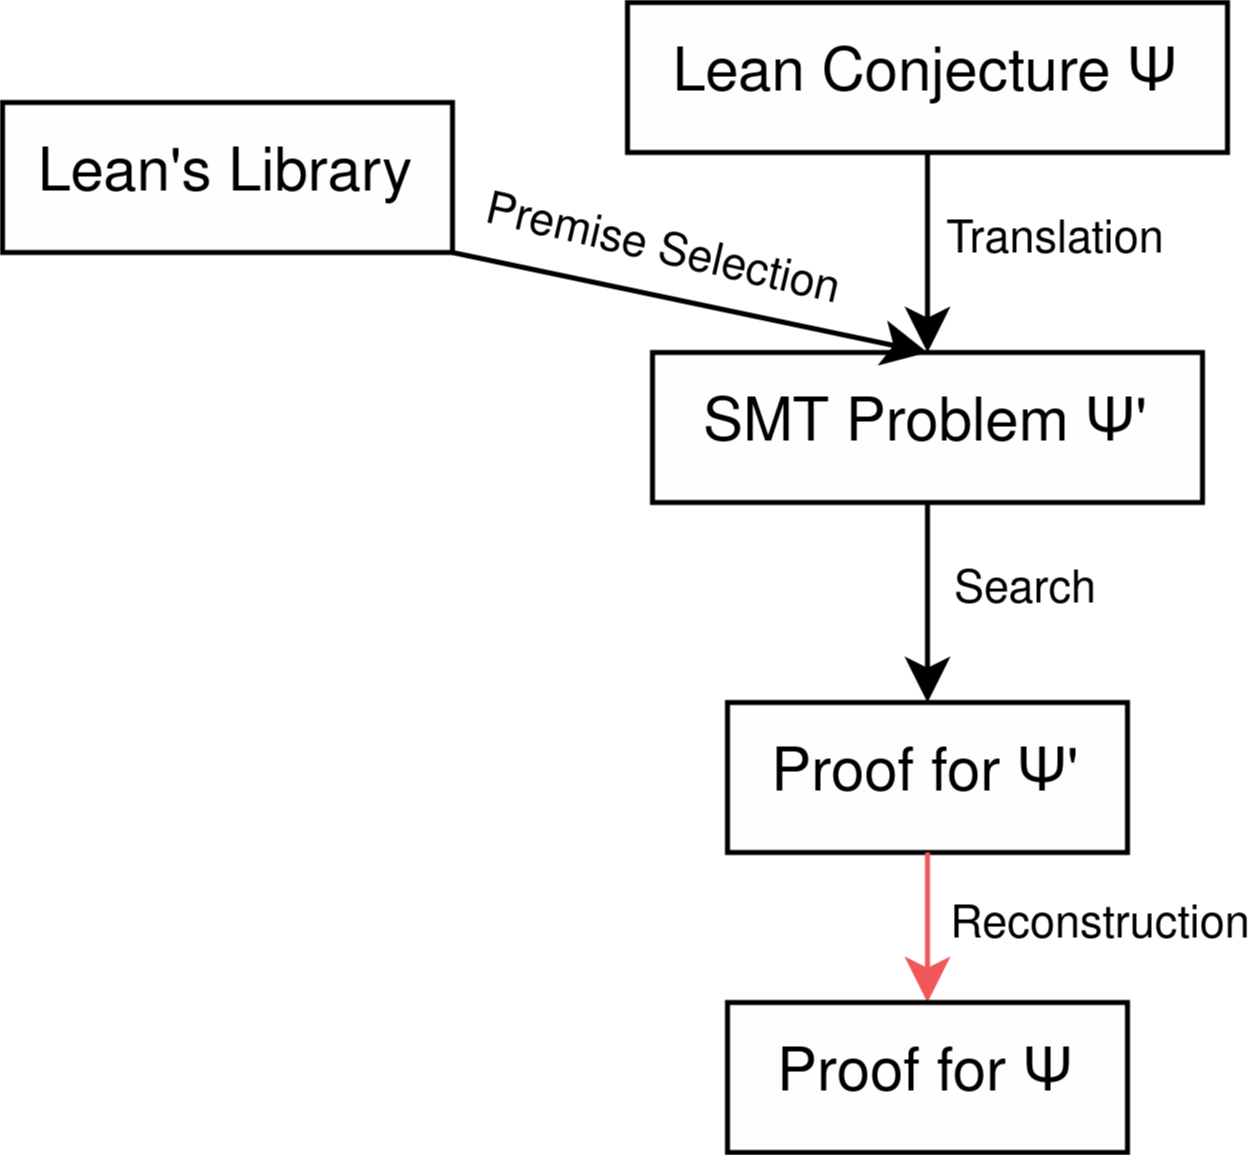
\includegraphics[height=0.65\textheight]{images/pic5.png}
  \end{minipage}
\end{frame}

\begin{frame}
  \frametitle{Implementing Hammers}
  \centering
  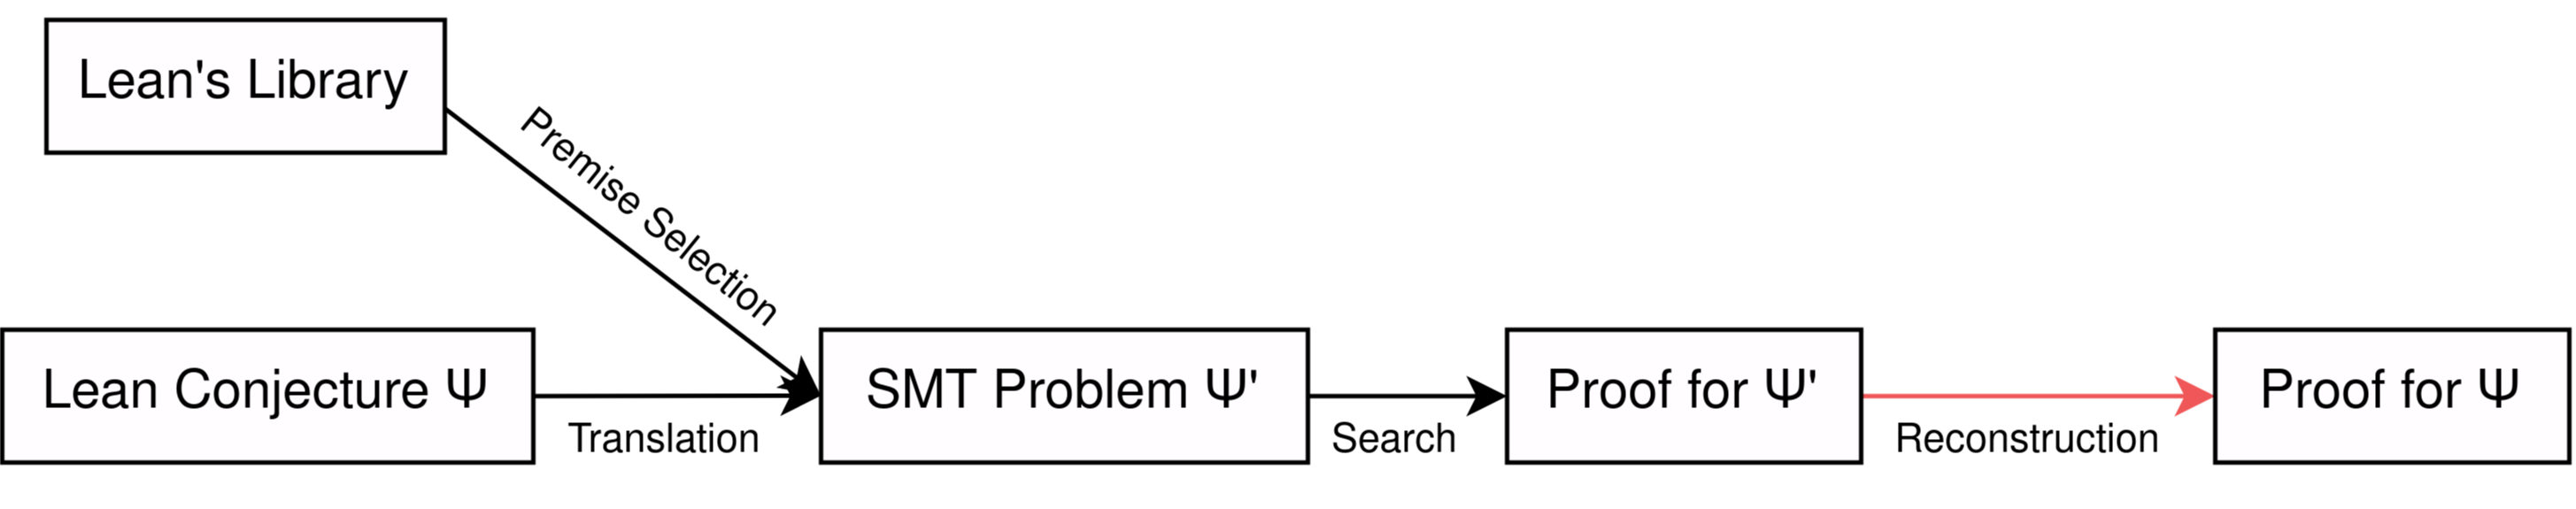
\includegraphics[height=0.3\textheight]{images/pic4.png}
\end{frame}

\begin{frame}
  \frametitle{Another Application}
  \begin{itemize}
    \item Checking results obtained by the ATP
    \begin{itemize}
      \item Carcara
    \end{itemize}
    \vitem Is the ITP reliable?
    \begin{itemize}
      \item Small kernel
      \item Many users constantly testing it
    \end{itemize}
    \vitem Is the certificate indeed proving the original theorem?
    \begin{itemize}
        \item If the theorem was printed wrongly, the proof would probably be incorrect
    \end{itemize}
  \end{itemize}
\end{frame}

\section{SMT Solvers}

\begin{frame}
  \frametitle{The SMT Problem}
  \begin{itemize}
    \item Boolean Satisfiability Problem (SAT)
    \vitem Decide whether a given formula built with boolean variables and the operators $\wedge$, $\vee$ and $\neg$ is satisfiable
  \end{itemize}
\end{frame}


\begin{frame}
  \frametitle{The SMT Problem}
  \begin{overprint}
    \onslide<1-2>
    \medskip
    $$\neg (x_{1} \vee x_{2}) \wedge x_{3} \wedge (\neg x_{1} \vee \neg x_{3})$$
  \end{overprint}
  \vfill
  \begin{overprint}
    \onslide<2>
    \begin{center}
      \textcolor{ForestGreen}{Satisfiable}\\
    $x_{1} \mapsto false$ \\
    $x_{2} \mapsto false$ \\
    $x_{3} \mapsto true$
    \end{center}
  \end{overprint}
\end{frame}

\begin{frame}
  \frametitle{The SMT Problem}
  \begin{overprint}
    \onslide<1-2>
    \medskip
    $$\neg (x_{1} \vee x_{2}) \wedge x_{3} \wedge (x_{1} \vee \neg x_{3})$$
  \end{overprint}
  \vfill
  \begin{overprint}
    \onslide<2>
    \begin{center}
      \color{red}Unsatisfiable
    \end{center}
  \end{overprint}
\end{frame}

\begin{frame}
  \frametitle{The SMT Problem}
  \begin{itemize}
    \item Satisfiability Modulo Theories is an extension over SAT
    \begin{itemize}
      \item We still want to check if formulas are satisfiable
    \end{itemize}
    \vitem Variables can range over different domains (sorts) apart from Boolean
    \vitem Operators from these domains are also added
    \vitem Theories of our interest:
    \begin{itemize}
      \item Equality and Uninterpreted Functions
      \item Linear Arithmetic
    \end{itemize}
    \vitem Many-Sorted First Order Logic (MSFOL)
  \end{itemize}
\end{frame}

\begin{frame}
  \frametitle{The SMT Problem}
  \begin{overprint}
    \onslide<1-2>
    \medskip
    \begin{center}
      $(x_{1} > x_{2}) \wedge (x_{2} \ge 0) \wedge (x_{1} < 2) \wedge (f(x_{1}) \not\simeq f(1) \vee x_{2} > 3)$ \\
      % $ (x_{1} \ge 0) \wedge (x_{1} < 2) \wedge (x_{1} \times x_{2} \not\simeq 0) \wedge ((f(5x_{1}) \not\simeq f(5)) \vee (x_{2} \simeq 0)) $ \\

      $x_{1}, x_{2} \in \mathbb{Z}$ \\

      $f : \mathbb{Z} \rightarrow \mathbb{Z}$
    \end{center}
  \end{overprint}
  \vfill
  \begin{overprint}
    \onslide<2>
    \begin{center}
      \color{red}Unsatisfiable
    \end{center}
  \end{overprint}
\end{frame}

\begin{frame}
  \frametitle{SMT Solvers}
  \begin{itemize}
    \item SMT Solvers are systems that aim to solve the SMT problem
    \vitem In order to determine whether a given formula is satisfiable, they combine SAT solvers with theory specific solvers
    \begin{itemize}
      \item Theory specific solvers only deal with conjunctions of propositions
    \end{itemize}
    \vitem Most of them accept the SMT-Lib format as input
  \end{itemize}
\end{frame}

\begin{frame}[fragile]
  \frametitle{SMT Solvers}
  \begin{minted}{smtlib.py -x}
    (set-logic QF_UFLIA)

    (declare-const x1 Int)
    (declare-const x2 Int)
    (declare-fun f (Int) Int)

    (assert (> x1 x2))
    (assert (>= x2 0))
    (assert (< x1 2))
    (assert (or (not (= (f x1) (f 1))) (> x2 3)))

    (check-sat)
  \end{minted}
\end{frame}

\begin{frame}
  \frametitle{SMT Solvers}
  \begin{itemize}
    \item Furthermore, some SMT solvers (including cvc5) can produce a proof certificate that supports the result found for a given formula
    \vitem For ``SAT'' results this is easy: just show the valuation of the variables
    \vitem What about ``UNSAT'' results?
  \end{itemize}
\end{frame}

% \begin{frame}
%   \frametitle{Proof Certificates for Boolean Formulas}
%   \begin{itemize}
%     \item Conjunctive Normal Form Transformation
%     \begin{itemize}
%       \item Representing the formula as a conjunction of clauses
%     \end{itemize}
%   \end{itemize}
%   \vfill
%       $$(x_{1} \vee \neg (x_{2} \wedge x_{3})) \wedge \neg (x_{1} \wedge \neg x_{4}) \Rightarrow (x_{1} \vee \neg x_{2} \vee \neg x_{3}) \wedge (\neg x_{1} \vee x_{4})$$
% \end{frame}

\begin{frame}
  \frametitle{Proof Certificates for Boolean Formulas}
    \begin{itemize}
    \item Assume that the input formula is in Conjunctive Normal Form (i.e. a conjunction of clauses)
    \vitem Resolution Rule
    \begin{itemize}
      \item Let $x$ be a variable and $C_{1}$ and $C_{2}$ be two clauses. If $x$ appears in $C_{1}$ and $\neg x$ appears in $C_{2}$, then from $C_{1} \wedge C_{2}$ we can conclude $C_{1}' \vee C_{2}'$, where $C_{1}'$ is $C_{1}$ without $x$ and $C_{2}'$ is $C_{2}$ without $\neg x$
    \end{itemize}
  \end{itemize}
          \vfill
          $$ (x_{1} \vee \neg x_{2} \vee \neg x_{3}) \wedge (x_{4} \vee \neg x_{1}) \Rightarrow \neg x_{2} \vee \neg x_{3} \vee x_{4} $$
\end{frame}

\begin{frame}
  \frametitle{Proof Certificates for Boolean Formulas}
  \begin{itemize}
    \item SAT solvers use the resolution rule to solve Boolean formulas in CNF
    \vitem They can be modified to register each instance of resolution applied while they are solving a problem, which will produce a \textit{resolution tree}
    \vitem Consider the formula $(x \vee y) \wedge (x \vee \neg y \vee z) \wedge (\neg x \vee z) \wedge  \neg z$. The following is a resolution tree certifying the unsatisfiability of this formula:
  \end{itemize}
  \vfill
  \[
\infer[]{\bot}{
  \infer[]
  {x}
  {x \vee y & \infer[]{x \vee \neg y}{x \vee \neg y \vee z & \neg z}} & \infer[]{\neg x}{\neg x \vee z & \neg z}}
\]
\end{frame}

\begin{frame}
  \frametitle{Proof Certificates for Boolean Formulas}
  \begin{itemize}
    \item If the input formula is \textbf{not} in CNF, the SAT solver applies a set of rules to transform it into a CNF formula
    \vitem These rules can also be captured in the same way as the resolution rule and embedded in the proof tree
  \end{itemize}
\end{frame}

\begin{frame}
  \frametitle{Proof Certificates for Boolean Formulas}
  \begin{itemize}
    \item Consider again the following unsatisfiable formula: $\neg (x_{1} \vee x_{2}) \wedge x_{3} \wedge (x_{1} \vee \neg x_{3})$
    \vitem By applying the \textit{De Morgan's Law} in the sub-expression $\neg (x_{1} \vee x_{2})$ we obtain $\neg x_{1} \wedge \neg x_{2}$
    \vitem Substituting it on the original formula, we obtain a CNF formula with 4 clauses: $\neg x_{1} \wedge \neg x_{2} \wedge x_{3} \wedge (x_{1} \vee \neg x_{3})$
  \end{itemize}

    \begin{prooftree}
      \AxiomC{$\neg (x_{1} \vee x_{2})$}
      \RightLabel{\footnotesize\textit{deMorgan}}
      \UnaryInfC{$\neg x_{1} \wedge \neg x_{2}$}
      \RightLabel{\footnotesize\textit{andElim}}
      \UnaryInfC{$\neg x_{1}$}

      \AxiomC{$x_{1} \vee \neg x_{3}$}
      \AxiomC{$x_{3}$}
      \RightLabel{\footnotesize\textit{resolution}}
      \BinaryInfC{$x_{1}$}
      \RightLabel{\footnotesize\textit{resolution}}
      \BinaryInfC{$\bot$}
    \end{prooftree}
\end{frame}

\begin{frame}
  \frametitle{Proof Certificates for Equality and Uninterpreted Functions}
  \begin{itemize}
    \item Next, we consider the theory of Equality and Uninterpreted Functions
    \vitem Variables can now also range over a special sort $U$ or be functions taking parameters from this sort
    \vitem We also introduce an equality operator: $\simeq$
    \vitem Examples:
  \end{itemize}
  \begin{enumerate}
    \item $(b \simeq c) \wedge (f(b) \simeq c) \wedge (f(c) \simeq a) \wedge (a \not\simeq b)$
    \item $(a \simeq f(f(a))) \wedge (a \simeq f(f(f(a)))) \wedge (f(a) \not\simeq a)$
  \end{enumerate}
\end{frame}

\begin{frame}
  \frametitle{Proof Certificates for Equality and Uninterpreted Functions}
  \begin{itemize}
    \item Function applications respect the congruence property:
    \begin{itemize}
      \item If $f$ and $g$ are two functions and $x$ and $y$ are two variables, $f \simeq g$ and $x \simeq y$ imply $f(x) \simeq g(y)$
      \item Extensionality
    \end{itemize}
    \vitem Proof certificates for unsatisfiability of formulas in this theory consist of proof trees in which the transitions are applications of congruence, reflexivity, symmetry and transitivity
  \end{itemize}
\end{frame}

\begin{frame}
  \frametitle{Proof Certificates for Equality and Uninterpreted Functions}
  \begin{itemize}
    \item Proof certificate for $(a \simeq f(f(a))) \wedge (a \simeq f(f(f(a)))) \wedge (f(a) \not\simeq a)$
  \end{itemize}
  \vfill
  \[
    \infer[\textit{resolution}]{\bot}{\infer[\textit{trans}]{f(a) \simeq a}{\infer[\textit{cong}]{f(a) \simeq f(f(f(a)))}{\infer[\textit{refl}]{f \simeq f}{} & a \simeq f(f(a))} & \infer[\textit{symm}]{f(f(f(a))) \simeq a}{a \simeq f(f(f(a)))}} & f(a) \not\simeq a}
  \]
\end{frame}

\begin{frame}
  \frametitle{Proof Certificates for Linear Arithmetic}
  \begin{itemize}
    \item In the theory of Linear Arithmetic, we consider numeric variables that can be added and scaled by constants
    \vitem Linear Integer Arithmetic vs Linear Real Arithmetic
    \vitem General form of a term:
  \end{itemize}
  \[
    \sum_{i} a_{i} x_{i} \bowtie b
  \]
  Where $\bowtie$ is either $<$, $\le$ or $\simeq$
\end{frame}

\begin{frame}
  \frametitle{Proof Certificates for Linear Arithmetic}
  \begin{itemize}
    \item Example: $x_{1} + x_{2} \le 1 \wedge 2x_{1} - 2x_{2} \le -4 \wedge x_{1} \ge 0 \wedge x_{2} \ge 0$
    \vitem Proof certificates for unsatisfiability of formulas in LRA rely on the Farkas' lemma:
    \begin{itemize}
      \item If there is no solution for a sequence of restrictions, then there is a sequence of coefficients $s_{i}$ such that one can derive an absurd by multiplying each coefficient to the corresponding restriction and adding all scaled restrictions
    \end{itemize}
    \vitem For the example above, one can multiply the first restriction by 2 and the second by 1 and add them to obtain $4x_{1} \le -3$, which is an absurd, since another restriction says that $x_{1} \ge 0$.
  \end{itemize}
\end{frame}

\begin{frame}
  \frametitle{Proof Certificates for Linear Arithmetic}
  \begin{itemize}
    \item Since the Farkas' lemma guarantee that such coefficients always exist, the SMT solver can compute them and provide it as a proof certificate.
    \vitem Linear Integer Arithmetic? Tight Bounds?
  \end{itemize}
\end{frame}

\section{Lean}

\begin{frame}
  \frametitle{Lean}
  \begin{itemize}
    \item Lean is both a programming language and a proof assistant
    \vitem Its features include
    % \begin{itemize}
    %   \item It implements the correspondence between propositions and types
    %   \item The proof checker and the type checker are the same piece of code, a kernel with less than 7500 lines
    % \end{itemize}
    \vitem Mathlib
  \end{itemize}
\end{frame}

\begin{frame}[fragile]
  \frametitle{Lean}
  \begin{minted}{lean}
    inductive Natural where
      | zero : Natural
      | succ : Natural -> Natural

    open Natural

    def add (n m : Natural) : Natural :=
      match n with
      | zero    => m
      | succ n' => succ (add n' m)

    notation x " + " y => add x y
  \end{minted}
\end{frame}

\begin{frame}[fragile]
  \frametitle{Lean}
  \begin{minted}[fontsize=\footnotesize]{lean}
  theorem add_zero : ∀ (n : Natural), (n + zero) = n :=
    fun n =>
      match n with
      | zero    => rfl
      | succ n' => congrArg succ (add_zero n')

  theorem add_succ : ∀ (n m : Natural),
      (n + succ m) = succ (n + m) := fun n m =>
    match n with
    | zero    => rfl
    | succ n' => congrArg succ (add_succ n' m)

  theorem add_comm : ∀ (n m : Natural), (n + m) = (m + n) := fun n m =>
    match n with
    | zero    => Eq.symm (add_zero m)
    | succ n' =>
      Eq.trans (congrArg succ (add_comm n' m)) (Eq.symm (add_succ m n'))
  \end{minted}
\end{frame}

\section{Certified Transformations}

\section{Certifying Transformations}

\section{Demo: Proof Checking}

\section{Demo: Lean-SMT}

% \maketitle

\end{document}

%%% Local Variables:
%%% mode: latex
%%% TeX-master: t
%%% End:
